\documentclass[a4paper]{article}

%%%%%%%% CREATE DOCUMENT STRUCTURE %%%%%%%%
%% Language and font encodings
\usepackage[english]{babel}
\usepackage[utf8x]{inputenc}
\usepackage[T1]{fontenc}
%\usepackage{subfig}

%% Sets page size and margins
\usepackage[a4paper,top=3cm,bottom=2cm,left=2cm,right=2cm,marginparwidth=1.75cm]{geometry}

%% Useful packages
\usepackage{amsmath,amssymb}
\usepackage{graphicx}
\usepackage[colorinlistoftodos]{todonotes}
\usepackage[colorlinks=true, allcolors=blue]{hyperref}
\usepackage{caption}
\usepackage{subcaption}
\usepackage{sectsty}
\usepackage{apacite}
\usepackage{float}
\usepackage{titling} 
\usepackage{blindtext}
\usepackage[square,sort,comma,numbers]{natbib}
\usepackage[colorinlistoftodos]{todonotes}
\usepackage{xcolor}
\definecolor{darkgreen}{rgb}{0.0, 0.4, 0.0}
\usepackage{graphicx}
\newcommand{\norm}[1]{\left\lVert#1\right\rVert}
\DeclareMathOperator{\R}{\mathbb{R}}
\DeclareMathOperator{\E}{\mathbb{E}}

\usepackage{listings}
\usepackage{xcolor}

\definecolor{codegreen}{rgb}{0,0.6,0}
\definecolor{codegray}{rgb}{0.5,0.5,0.5}
\definecolor{codepurple}{rgb}{0.58,0,0.82}
\definecolor{backcolour}{rgb}{0.95,0.95,0.92}

\lstdefinestyle{mystyle}{
	backgroundcolor=\color{backcolour},   
	commentstyle=\color{codegreen},
	keywordstyle=\color{magenta},
	numberstyle=\tiny\color{codegray},
	stringstyle=\color{codepurple},
	basicstyle=\ttfamily\footnotesize,
	breakatwhitespace=false,         
	breaklines=true,                 
	captionpos=b,                    
	keepspaces=true,                 
	numbers=left,                    
	numbersep=5pt,                  
	showspaces=false,                
	showstringspaces=false,
	showtabs=false,                  
	tabsize=2
}

\lstset{style=mystyle}
 



%%%%%%%% DOCUMENT %%%%%%%%
\begin{document}

%%%% Title Page
\begin{titlepage}

\newcommand{\HRule}{\rule{\linewidth}{0.5mm}} 							% horizontal line and its thickness
\center 
 
 
% University


\includegraphics[width=0.15\textwidth]{images/kth_logo.png}\\[0.5cm] 	% University logo

\textsc{\LARGE KTH Royal Institute of Technology}\\[1cm]

% Document info
\textsc{\Large Deep Learning in Datascience}\\[0.2cm]
\textsc{\large DD2424}\\[1cm] 										% Course Code
\HRule \\[0.8cm]
{ \huge \bfseries Assignment 3}\\[0.7cm]								% Assignment
\HRule \\[2cm]
\large
\emph{Authors:}\\
Ali Banaei Mobarak Abadi\\[1.5cm]													% Author info
{\large \today}\\[5cm]

\vfill 
\end{titlepage}

%%\begin{abstract}
%%Your abstract.
%%\end{abstract}

%%%% SECTIONS
%% Section 1
\section{Extending the code}

As the first step of this assignment, we had to generalize the code from the previous assignment to a k-layer multi-layer perceptron. In order to make the code easier to debug and more readable, I used an object-oriented approach to solve the problem. The \lstinline[basicstyle=\color{red}]{Model} class implements an MLP model by using \lstinline[basicstyle=\color{red}]{Dense_layer} class. In \lstinline[basicstyle=\color{red}]{Dense_layer} class, we have forward and backward methods. In the \lstinline[basicstyle=\color{red}]{forward} method, the layer performs the forward pass operation and stores the values it will need for calculating the gradient later. In \lstinline[basicstyle=\color{red}]{backward} method, the gradients of the cost function based on different components are calculated and stored. The gradient with respect to the inputs is returned to be used as input in the \lstinline[basicstyle=\color{red}]{backward} function of the previous layer. Also, I used He initialization for the initial values of the weights, and the initial value for $\gamma$ and $\beta$ are 1 and 0.


\section{Checking the gradient}

After implementing everything, the first step is to check if the calculation of the gradients is correctly implemented. So, all the gradients are compared to the numerically calculated versions to ensure implementation is bug-free. In order to make the comparison of values easier, the initial values of the weight vectors are changed to random values drawn from a normal distribution with a mean of 0 and a standard deviation equal to 2. By doing this, the values in the network will get big, and we will see big gradients. Also, if there is a bug in the implementation with big weights, the error will be amplified. Finally, we compare the mean, STD, and the max value of the difference between the two methods with the respective metrics of the gradient. The results of this comparison can be found in \autoref{lst:gradient}.

\begin{lstlisting}[label={lst:gradient}]
	model with no batch norm
	layer 0:
	W: mean=-0.5097001036303636 std=1.2106800385111829 mean_diff=9.95608131190151e-07 std_diff=1.3946208283390884e-06 max_diff=4.213600700575526e-06
	b: mean=0.6897851405067021 std=0.9101289248052089 mean_diff=6.026841938538974e-07 std_diff=7.496373064288024e-07 max_diff=2.0435311541555645e-06
	-----------
	layer 1:
	W: mean=0.5049977166998967 std=4.072281517260328 mean_diff=1.360864474285961e-05 std_diff=4.3855519461204086e-05 max_diff=0.00020874103731571836
	b: mean=0.2988415389271323 std=0.4954698414899397 mean_diff=2.4581335669113246e-07 std_diff=2.3652371620016618e-07 max_diff=6.637855751723265e-07
	-----------
	layer 2:
	W: mean=0.0043824488585420054 std=2.3629288066516163 mean_diff=1.4869869114031258e-06 std_diff=6.499394877309395e-06 max_diff=3.327843577949352e-05
	b: mean=-5.551115123125783e-18 std=0.167084261083203 mean_diff=9.947598307721243e-09 std_diff=1.0942000451612945e-08 max_diff=2.7732373175659575e-08
	-----------
	model with batch norm
	layer 0:
	W: mean=-0.0839780101579187 std=0.1771482696455477 mean_diff=8.939838169269576e-08 std_diff=2.441997646496221e-07 max_diff=1.0027733415851614e-06
	b: mean=-5.8286708792820724e-18 std=4.165556196590227e-17 mean_diff=-1.0658140978114796e-09 std_diff=1.4210854339113955e-09 max_diff=0.0
	gamma: mean=1.897402009967686e-07 std=0.9800554661835622 mean_diff=5.112102078305703e-07 std_diff=1.2930831486309136e-06 max_diff=3.067726149552641e-06
	betas: mean=0.24747773473014822 std=0.7069369348475908 mean_diff=-3.630722163472377e-08 std_diff=3.8770300560018024e-07 max_diff=7.235364460900229e-07
	-----------
	layer 1:
	W: mean=-0.09192297948795643 std=0.19137018135060274 mean_diff=1.552730084335152e-08 std_diff=9.923212471724819e-08 max_diff=3.405460177186015e-07
	b: mean=-2.9976021664879216e-17 std=7.487114753582493e-17 mean_diff=-7.105427057840785e-10 std_diff=8.702335314144054e-10 max_diff=4.4408920985006264e-17
	gamma: mean=0.8582151925485121 std=0.799033358393596 mean_diff=1.1782459954264024e-07 std_diff=8.254835598673965e-08 max_diff=2.613252086947071e-07
	betas: mean=0.9834085325781471 std=0.9216490070331642 mean_diff=3.147544647627565e-07 std_diff=2.7654333219880184e-07 max_diff=8.266876407869717e-07
	-----------
	layer 2:
	W: mean=-8.750016372312291e-05 std=0.13849091546221962 mean_diff=1.7573662150298896e-08 std_diff=1.8928908162452413e-08 max_diff=9.83173368551693e-08
	b: mean=1.1102230246251566e-17 std=0.1767370838506264 mean_diff=2.0250467958494307e-08 std_diff=2.177676795353542e-08 max_diff=7.629055043256727e-08
	-----------
\end{lstlisting}

As we can see, the differences are minimal compared to the actual values, and they are probably due to a numerical error in floating-point calculations.  Note that the gradients are for a three-layer network with the input size equal to 10. A bigger input size with big weights would result in floating-point overflow in calculations. So, we can conclude the implementation for both with and without batch normalization seems to work fine.


\section{Training the network}

In the next step, we try to train the model. The model is trained by the settings of exercise 2 with two hidden layers. \autoref{fig:3layer_no_bn} depicts the logs during the training. After training for two cycles, we reached the accuracy of 0.536 on validation and 0.529 on test data which is the same as the reported values in assignment instructions.

\begin{figure}[h]
	\centering
	\begin{subfigure}{0.3\textwidth}
		\centering
		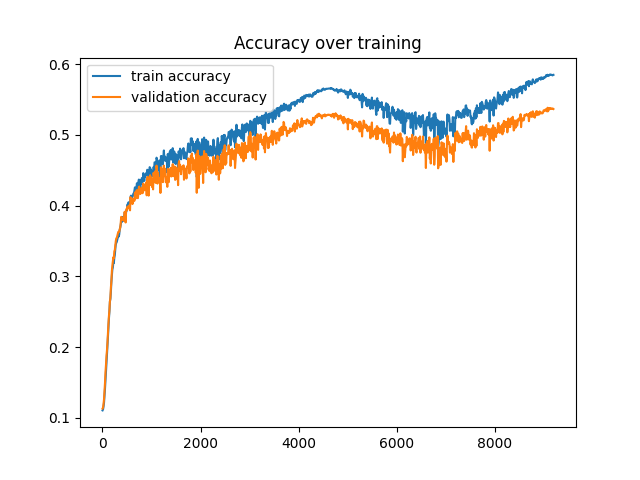
\includegraphics[width=\linewidth]{images/ex2_no_batch_acc.png}
		\caption{accuracy}
	\end{subfigure}
	\begin{subfigure}{0.3\textwidth}
		\centering
		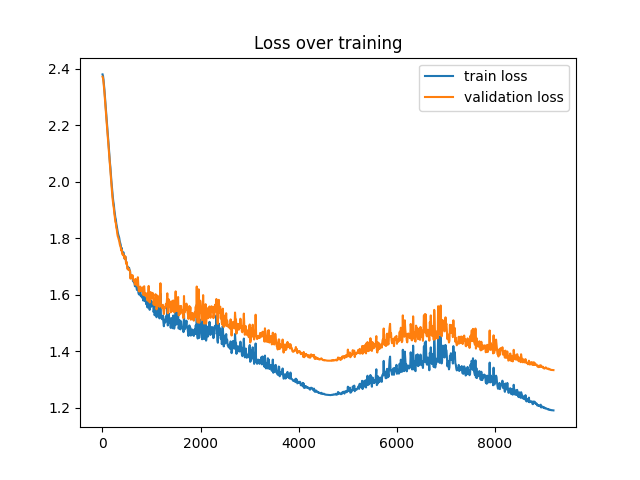
\includegraphics[width=\linewidth]{images/ex2_no_batch_loss.png}
		\caption{loss}
	\end{subfigure}
	\begin{subfigure}{0.3\textwidth}
		\centering
		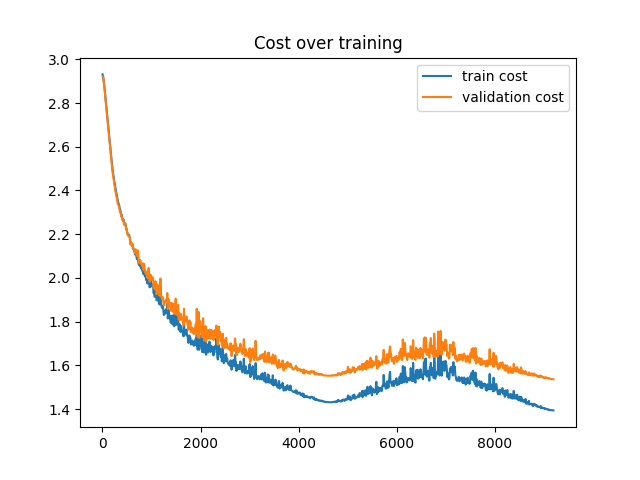
\includegraphics[width=\linewidth]{images/ex2_no_batch_cost.png}
		\caption{cost}
	\end{subfigure}
	\caption{Accuracy, loss and cost function for three-layer model of exercise 2.}
	\label{fig:3layer_no_bn}
\end{figure}

Then we must train the 9-layer model. With the same hyper-parameter settings, this model reached the accuracy of 0.461 on validation and 0.463 on test data. Logs of the training for this function can be found in \autoref{fig:9layer_no_bn}. As expected, with increasing the number of layers, we see a notable decrease in the performance of the network.

\begin{figure}[h]
	\centering
	\begin{subfigure}{0.3\textwidth}
		\centering
		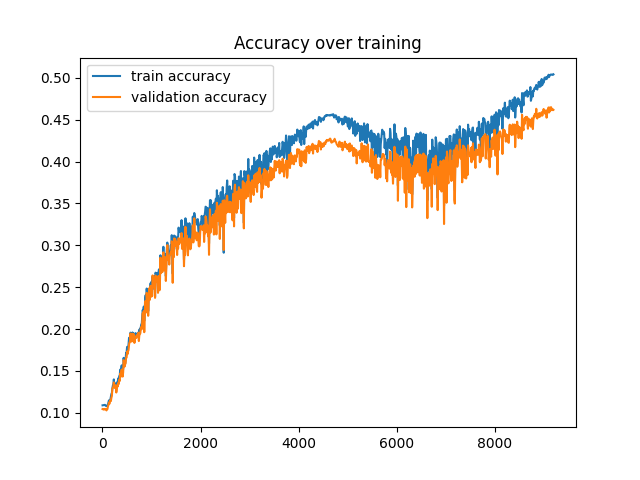
\includegraphics[width=\linewidth]{images/ex2_9layer_no_batch_acc.png}
		\caption{accuracy}
	\end{subfigure}
	\begin{subfigure}{0.3\textwidth}
		\centering
		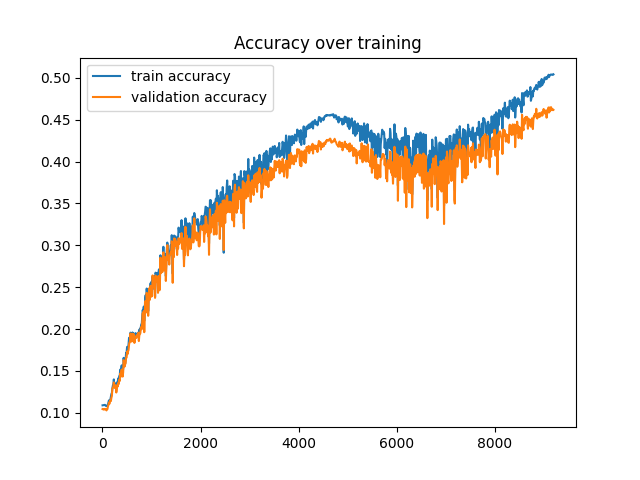
\includegraphics[width=\linewidth]{images/ex2_9layer_no_batch_acc.png}
		\caption{loss}
	\end{subfigure}
	\begin{subfigure}{0.3\textwidth}
		\centering
		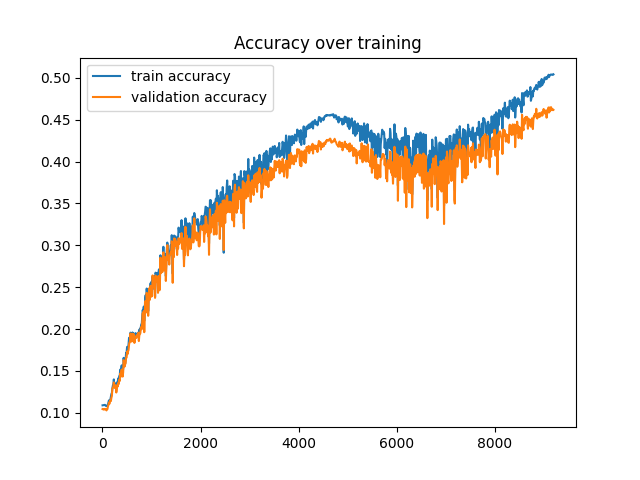
\includegraphics[width=\linewidth]{images/ex2_9layer_no_batch_acc.png}
		\caption{cost}
	\end{subfigure}
	\caption{Accuracy, loss and cost function for nine-layer model of exercise 2.}
	\label{fig:9layer_no_bn}
\end{figure}

\section{Batch Normalization}

Now that we have seen how a k-layer MLP performs on classification on CIFAR-10, it is time to test our network with Batch Normalization. We have already implemented it and tested the calculation of the gradients.
For the first step, we add batch normalization to the first and second layers of the three-layer architecture of the previous section. After training with the same settings as before, the network reached the accuracy of 0.542 on validation and 0.534 on test data. Logs are also available in \autoref{fig:3layer_with_bn}. As we saw, there is an small improvement on the performance of the network.

\begin{figure}[h]
	\centering
	\begin{subfigure}{0.3\textwidth}
		\centering
		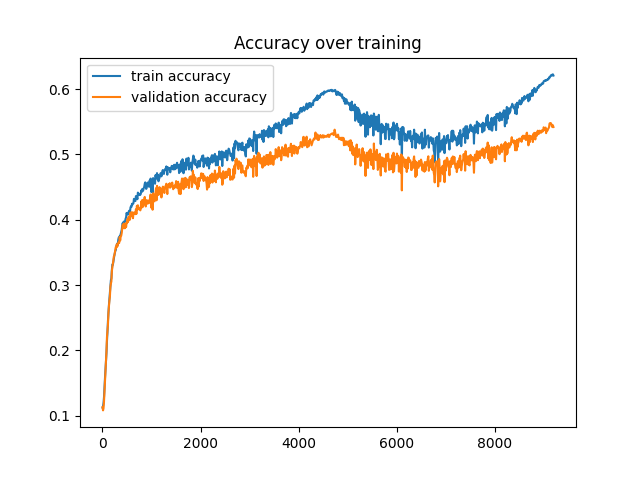
\includegraphics[width=\linewidth]{images/ex2_with_batch_acc.png}
		\caption{accuracy}
	\end{subfigure}
	\begin{subfigure}{0.3\textwidth}
		\centering
		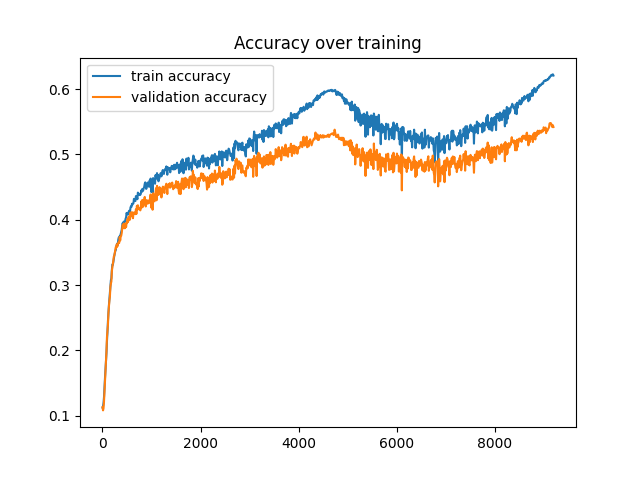
\includegraphics[width=\linewidth]{images/ex2_with_batch_acc.png}
		\caption{loss}
	\end{subfigure}
	\begin{subfigure}{0.3\textwidth}
		\centering
		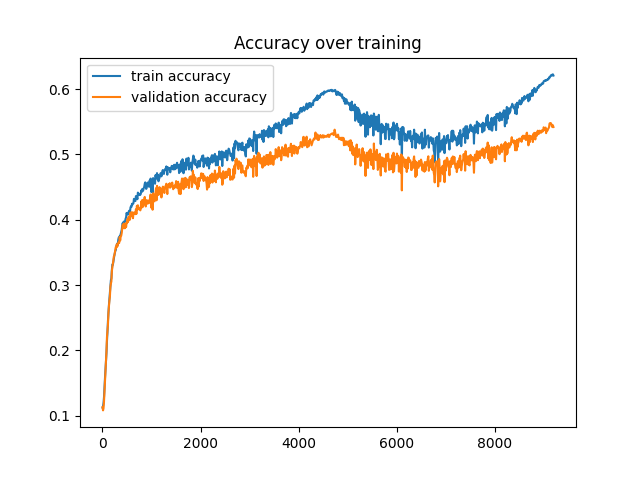
\includegraphics[width=\linewidth]{images/ex2_with_batch_acc.png}
		\caption{cost}
	\end{subfigure}
	\caption{Accuracy, loss and cost function for three-layer model of exercise 2 with batch normalization.}
	\label{fig:3layer_with_bn}
\end{figure}

The increase in final accuracy for the deeper model was more significant. After training, the performance of the 9-layer model was 0.524 on validation and 0.525 on test data. As we saw, it is still less than the model with fewer number of layers, but there is approximately a \%7 increase in the final accuracy. Logs of trainig can be found in \autoref{fig:9layer_with_bn}.




\begin{figure}[h]
	\centering
	\begin{subfigure}{0.3\textwidth}
		\centering
		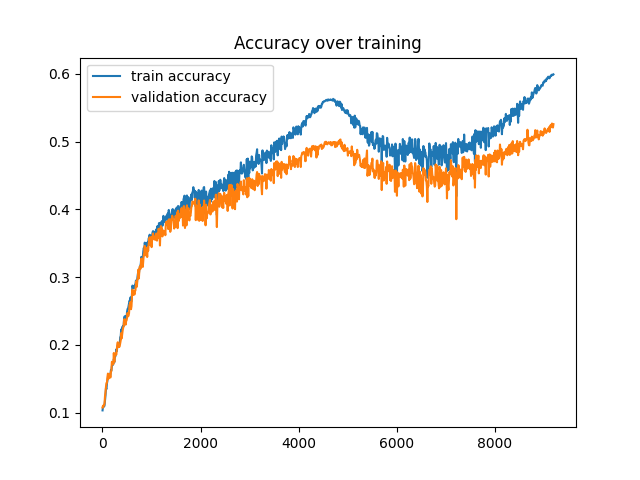
\includegraphics[width=\linewidth]{images/ex2_with_batch_9layer_acc.png}
		\caption{accuracy}
	\end{subfigure}
	\begin{subfigure}{0.3\textwidth}
		\centering
		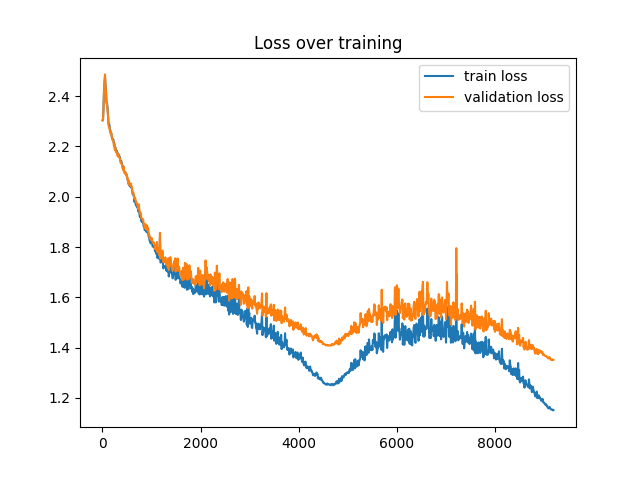
\includegraphics[width=\linewidth]{images/ex2_with_batch_9layer_loss.png}
		\caption{loss}
	\end{subfigure}
	\begin{subfigure}{0.3\textwidth}
		\centering
		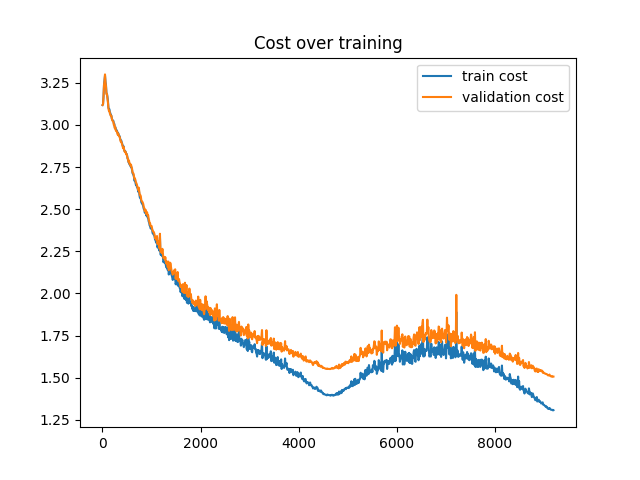
\includegraphics[width=\linewidth]{images/ex2_with_batch_9layer_cost.png}
		\caption{cost}
	\end{subfigure}
	\caption{Accuracy, loss and cost function for nine-layer model of exercise 2 with batch normalization.}
	\label{fig:9layer_with_bn}
\end{figure}

\section{Searching for $\lambda$}

In order to find a good value for the $\lambda$ parameter, we tried different values of $\lambda$ and trained the network for eight epochs (which is equal to the shorter training version in instructions). Then the validation accuracy was recorded for each setting. \autoref{tab:lambda} shows these values. As we can see, our three-layer network best performed when we trained it with very small $\lambda$ or even no regularization at all. This is interesting since, in the last assignment, we found that without using regularization, the network overfits very quickly, but here we do not see a sign of overfitting so far. This may indicate the regularization effect of batch normalization. Also, the performance of the best network with 8 epochs of training was 0.528 on the test data.

\begin{table}[h]
	\centering
	\caption{Validation accuracy for different values of $\lambda$.}
	\label{tab:lambda}
	\begin{tabular}{|l|l|} 
		\hline
		$sigma$ & Test accuracy without BN  \\ 
		\hline
		0.1                       & 0.464                     \\ 
		\hline
		0.05                      & 0.486                     \\ 
		\hline
		0.01                      & 0.515                     \\ 
		\hline
		0.005                     & 0.519                     \\ 
		\hline
		0.001                     & 0.514                     \\ 
		\hline
		0.0001                    & 0.522                     \\ 
		\hline
		0                         & 0.522                     \\
		\hline
	\end{tabular}
\end{table}







\section{Initialization sensitivity}

To investigate the effect of weight initialization, we used trained and tested the three-layer network with and without batch normalization with three different values for the $sigma$ value of the normal distribution which we sample from. Results can be seen in [].

As we see, when we have small values of $\sigma$, since the weights and thus the resulting outputs and gradients are small, the network is not able to learn and does a random classification. However, batch normalization with scaling the output makes the network more robust to initial values and results in normal learning even when the initial values are very small. The results of the evaluation on the test set can be found in \autoref{tab:init}. Logs during training for model with no use of batch normalization can be found in \autoref{fig:sens_no_bn} and \autopageref{fig:sens_bn} for model with batch normalization.

\begin{table}[h]
	\centering
	\caption{Test accuracy on three-layer network with different $\sigma$ values for random initialization.}
	\label{tab:init}
	\begin{tabular}{|l|l|l|} 
		\hline
		$\sigma$ & Test accuracy without BN & Test accuracy with BN  \\ 
		\hline
		0.1                       & 0.512                    & 0.522                  \\ 
		\hline
		1e-3                      & 0.1                      & 0.524                  \\ 
		\hline
		1e-4                      & 0.1                      & 0.527                  \\
		\hline
	\end{tabular}
\end{table}


\begin{figure}[h]
	\centering
	\begin{subfigure}{0.3\textwidth}
		\centering
		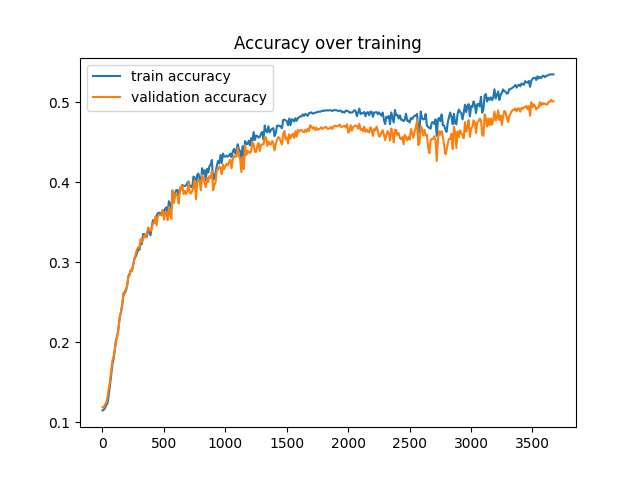
\includegraphics[width=\linewidth]{images/sens_sigma_0.1_use_bn_False_acc.png}
		\caption{accuracy $\sigma=0.1$}
	\end{subfigure}
	\begin{subfigure}{0.3\textwidth}
		\centering
		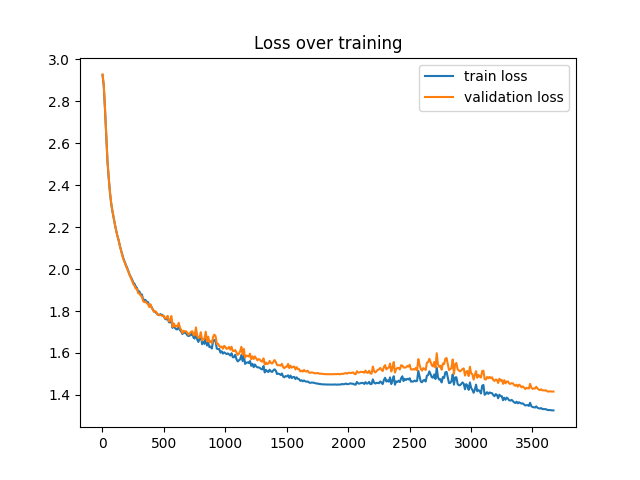
\includegraphics[width=\linewidth]{images/sens_sigma_0.1_use_bn_False_loss.png}
		\caption{loss $\sigma=0.1$}
	\end{subfigure}
	\begin{subfigure}{0.3\textwidth}
		\centering
		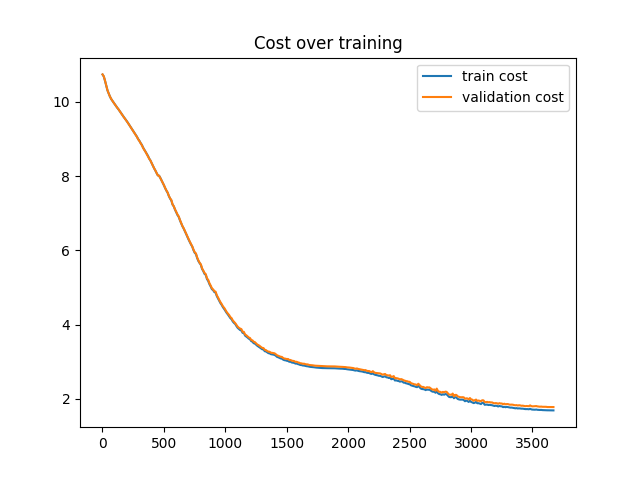
\includegraphics[width=\linewidth]{images/sens_sigma_0.1_use_bn_False_cost.png}
		\caption{cost $\sigma=0.1$}
	\end{subfigure} \\
	
	\begin{subfigure}{0.3\textwidth}
		\centering
		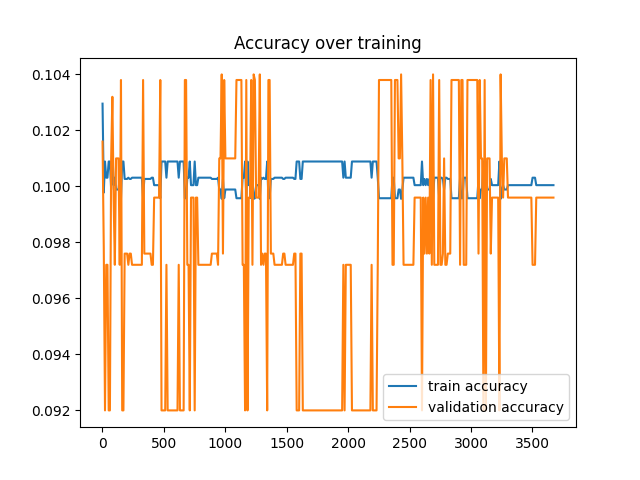
\includegraphics[width=\linewidth]{images/sens_sigma_0.001_use_bn_False_acc.png}
		\caption{accuracy $\sigma=1e-3$}
	\end{subfigure}
	\begin{subfigure}{0.3\textwidth}
		\centering
		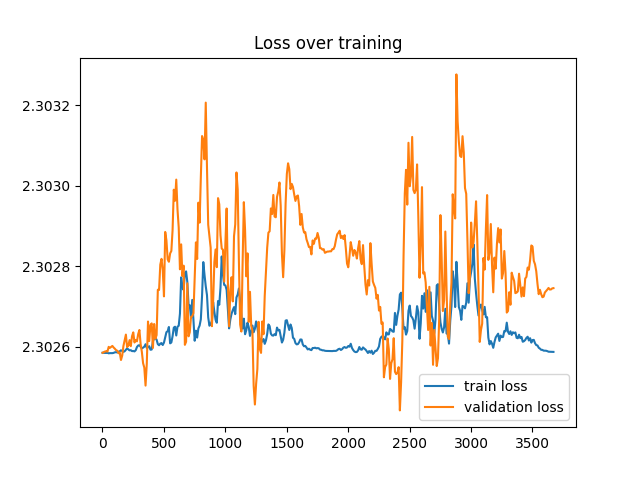
\includegraphics[width=\linewidth]{images/sens_sigma_0.001_use_bn_False_loss.png}
		\caption{loss $\sigma=1e-3$}
	\end{subfigure}
	\begin{subfigure}{0.3\textwidth}
		\centering
		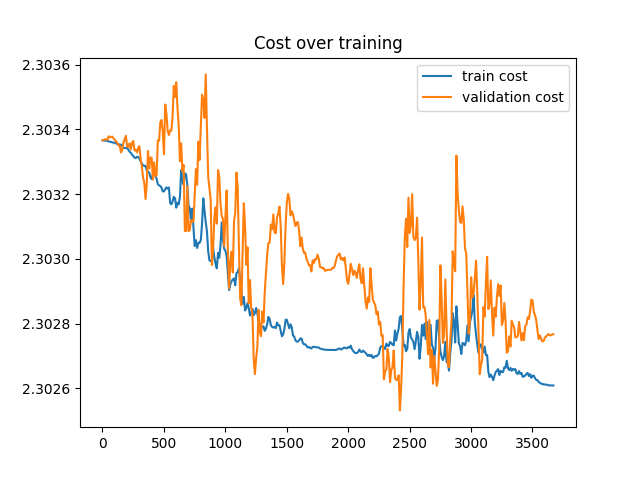
\includegraphics[width=\linewidth]{images/sens_sigma_0.001_use_bn_False_cost.png}
		\caption{cost $\sigma=1e-3$}
	\end{subfigure} \\

	\begin{subfigure}{0.3\textwidth}
		\centering
		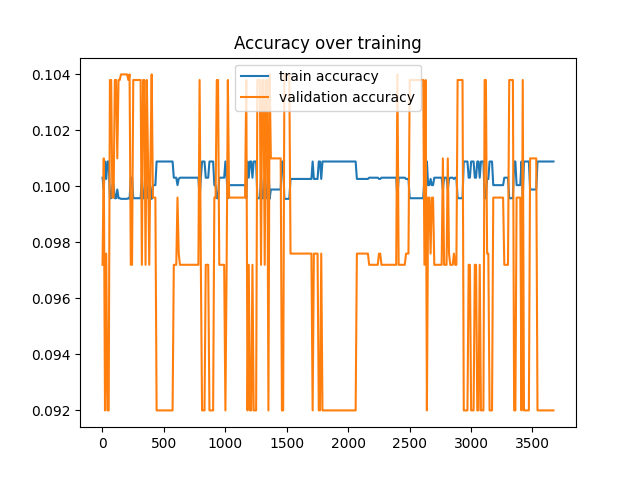
\includegraphics[width=\linewidth]{images/sens_sigma_0.0001_use_bn_False_acc.png}
		\caption{accuracy $\sigma=1e-4$}
	\end{subfigure}
	\begin{subfigure}{0.3\textwidth}
		\centering
		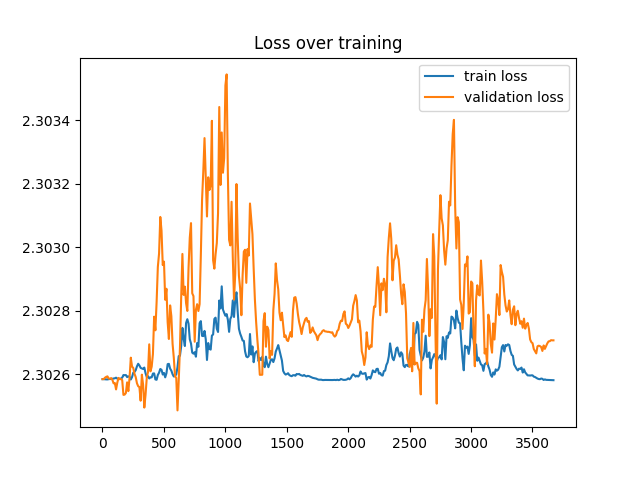
\includegraphics[width=\linewidth]{images/sens_sigma_0.0001_use_bn_False_loss.png}
		\caption{loss $\sigma=1e-4$}
	\end{subfigure}
	\begin{subfigure}{0.3\textwidth}
		\centering
		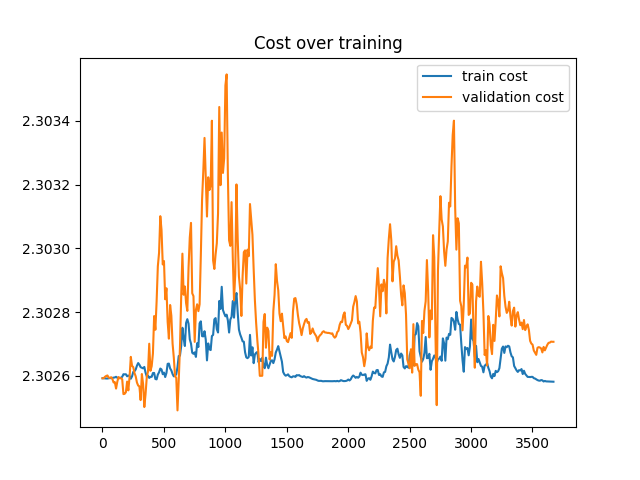
\includegraphics[width=\linewidth]{images/sens_sigma_0.0001_use_bn_False_cost.png}
		\caption{cost $\sigma=1e-4$}
	\end{subfigure} \\

	\caption{Accuracy, loss and cost function for three-layer model of exercise 2 without batch normalization and sifferent $\sigma$ values.}
	\label{fig:sens_no_bn}
\end{figure}


\begin{figure}[h]
	\centering
	\begin{subfigure}{0.3\textwidth}
		\centering
		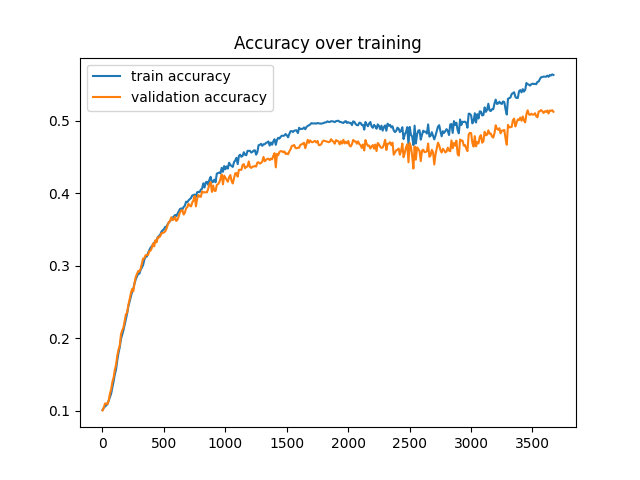
\includegraphics[width=\linewidth]{images/sens_sigma_0.1_use_bn_True_acc.png}
		\caption{accuracy $\sigma=0.1$}
	\end{subfigure}
	\begin{subfigure}{0.3\textwidth}
		\centering
		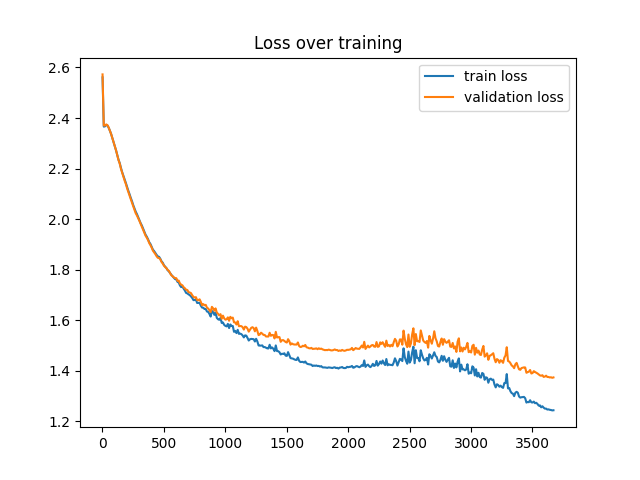
\includegraphics[width=\linewidth]{images/sens_sigma_0.1_use_bn_True_loss.png}
		\caption{loss $\sigma=0.1$}
	\end{subfigure}
	\begin{subfigure}{0.3\textwidth}
		\centering
		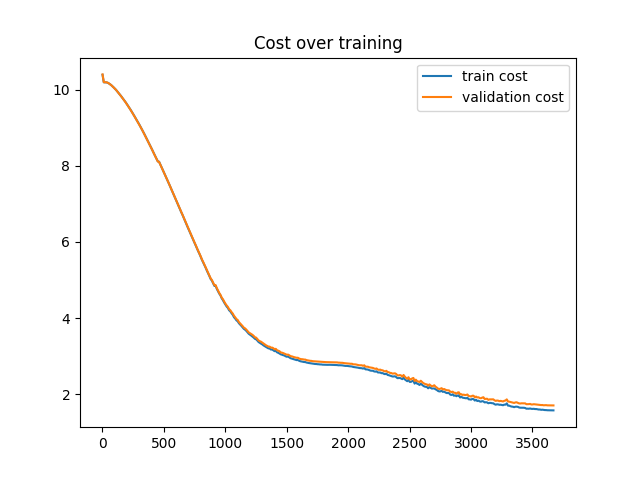
\includegraphics[width=\linewidth]{images/sens_sigma_0.1_use_bn_True_cost.png}
		\caption{cost $\sigma=0.1$}
	\end{subfigure} \\
	
	\begin{subfigure}{0.3\textwidth}
		\centering
		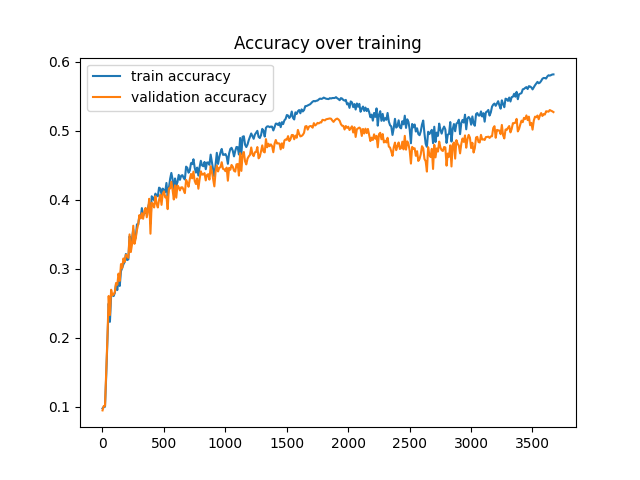
\includegraphics[width=\linewidth]{images/sens_sigma_0.001_use_bn_True_acc.png}
		\caption{accuracy $\sigma=1e-3$}
	\end{subfigure}
	\begin{subfigure}{0.3\textwidth}
		\centering
		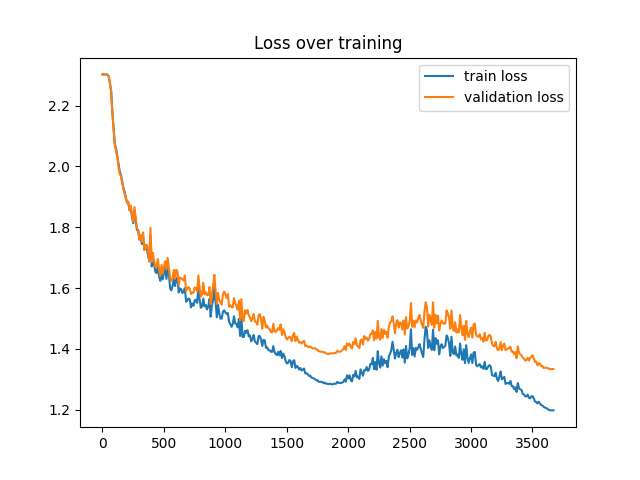
\includegraphics[width=\linewidth]{images/sens_sigma_0.001_use_bn_True_loss.png}
		\caption{loss $\sigma=1e-3$}
	\end{subfigure}
	\begin{subfigure}{0.3\textwidth}
		\centering
		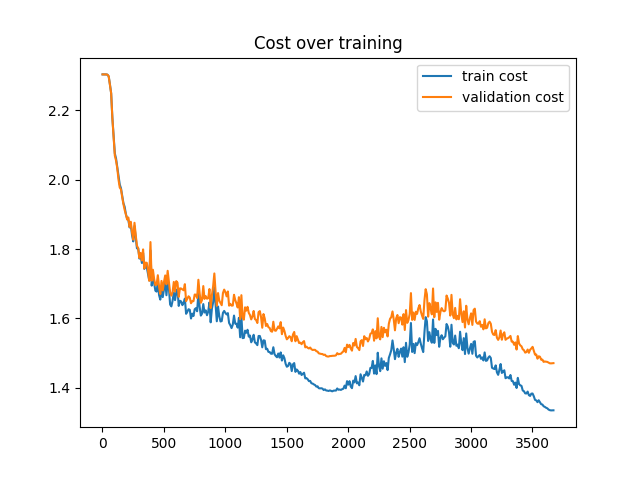
\includegraphics[width=\linewidth]{images/sens_sigma_0.001_use_bn_True_cost.png}
		\caption{cost $\sigma=1e-3$}
	\end{subfigure} \\
	
	\begin{subfigure}{0.3\textwidth}
		\centering
		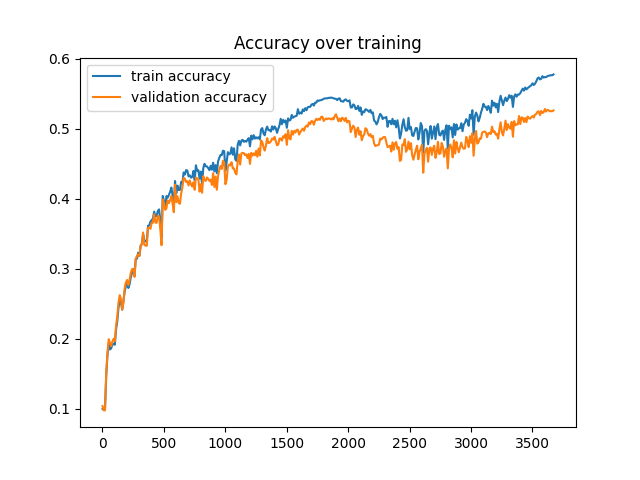
\includegraphics[width=\linewidth]{images/sens_sigma_0.0001_use_bn_True_acc.png}
		\caption{accuracy $\sigma=1e-4$}
	\end{subfigure}
	\begin{subfigure}{0.3\textwidth}
		\centering
		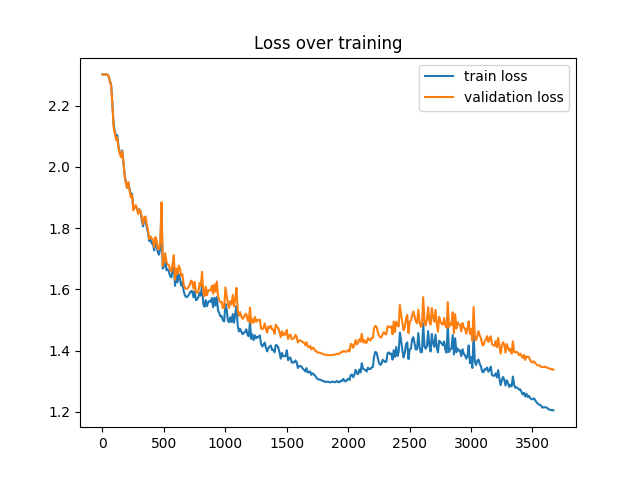
\includegraphics[width=\linewidth]{images/sens_sigma_0.0001_use_bn_True_loss.png}
		\caption{loss $\sigma=1e-4$}
	\end{subfigure}
	\begin{subfigure}{0.3\textwidth}
		\centering
		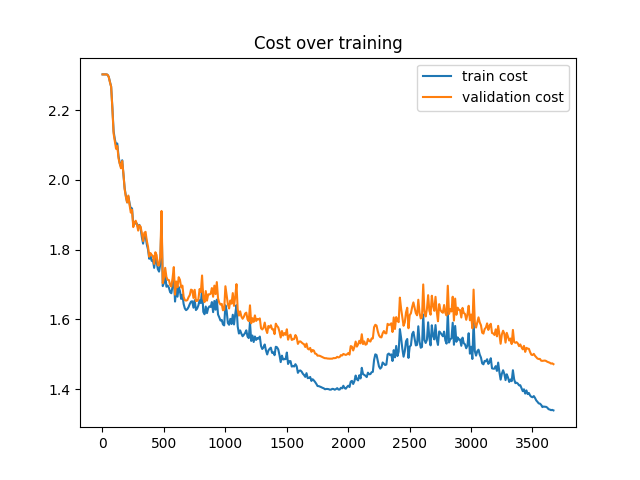
\includegraphics[width=\linewidth]{images/sens_sigma_0.0001_use_bn_True_cost.png}
		\caption{cost $\sigma=1e-4$}
	\end{subfigure} \\
	
	\caption{Accuracy, loss and cost function for three-layer model of exercise 2 with batch normalization and sifferent $\sigma$ values.}
	\label{fig:sens_bn}
\end{figure}

%%%%%%%% EXTRA TIPS %%%%%%%%
%% If you want to include an figure
%%\begin{figure}[H]
%%\includegraphics[]{Pendulum.jpg}
%%\caption{Sketch of the pendulum}
%%\label{fig:pendulum}
%%\end{figure}

%% for multiple figures in one fig
%\begin{figure}[h]
%	\centering
%	\begin{subfigure}{\textwidth}
%		\centering
%		\includegraphics[width=\linewidth]{images/sthfivo.png}
%		\caption{}
%	\end{subfigure}
%	\begin{subfigure}{\textwidth}
%		\centering
%		\includegraphics[width=\linewidth]{images/sth.png}
%		\caption{}
%	\end{subfigure}
%	\begin{subfigure}{\textwidth}
%		\centering
%		\includegraphics[width=\linewidth]{images/sth.png}
%		\caption{}
%	\end{subfigure}
%	\caption{caption}
%	\label{fig:label}
%\end{figure}


%% You can then reference with \ref{fig:pendulum}


%%\newpage
%\bibliographystyle{apacite}
%\bibliography{ref.bib}

\end{document}